%%%%%%%%%%
% [TODO] %
%%%%%%%%%%
% [ ] Better figures for the annexes 
% [ ] Add correlation ABX-id
% [ ] Figure captions

%%%%%%%%%%%%%%%%%%%%%%
% Chapter mini-intro %
%%%%%%%%%%%%%%%%%%%%%%

%% Short background %%

[Short BG] \\

%% Research questions (+ alternatives) %%

[Research questions] \\

%% Plan %%

In \textbf{section 2.1} a perceptual experiment aims to disentangle the contributions of phonetic categories and acoustic details on epenthetic vowel quality. Participants are asked to report their choice of epenthetic vowel (if any) within consonant cluster in stimuli where the acoustic information contained in the cluster may be in disagreement with the identity of neighbouring vowels. Information theoretic measures allow to quantify the influence of both neighbouring phonetic categories and acoustic details.  


In \textbf{section 2.2} I investigate the possibility of predicting epenthetic vowel quality in Brazilian Portuguese (BP) and Japanese (JP) using a production-based exemplar model of perception. This type of model predicts the quality of a vowel epenthesized within the cluster of a stimulus based solely on the acoustic similarity of said /CC/ cluster to /CVC/ exemplars produced by native speakers of BP or JP. From this modelling approach we can evaluate the influence of pure acoustics on effects such as default epenthetic vowel quality and modulations induced by neighbouring vowels.

%%%%%%%%%%%%%%%%%%%%
% /ahpa/ (JASA-EL) %
%%%%%%%%%%%%%%%%%%%%

%%%% Main %%%%
\includepdf[pages={2-8}, pagecommand={},
addtotoc={
  2,section,1,Which epenthetic vowel? \\ Phonetic categories versus acoustic detail in perceptual vowel epenthesis,ahpa_main,
  3,subsection,2,Methods,ahpa_methods,
  4,subsection,2,Results,ahpa_results,
  6,subsection,2,Discussion,ahpa_disc,
  7,subsection,2,References,ahpa_ref}]
{images/chapter02/JASAEL_Guevara-Rukoz_2017_Which_epenthetic_vowel.pdf}

%%%% Annexes %%%%
\subsection{Annexes}

\subsubsection{Acoustic analyses}
\begin{figure}[H]
  \centering
  \begin{overpic}[page=1, width=0.8\linewidth]{chapter02/ahpa_acoustic}\end{overpic}
  \caption{Figure caption}
  \label{fig:ahpa_acoustic}
\end{figure}

\subsubsection{Control items}
\begin{figure}[H]
  \centering
  \begin{overpic}[page=1, width=0.2\linewidth]{chapter02/ahpa_uep-copyep}\end{overpic}
  \hspace{2cm}
  \begin{overpic}[page=2, width=0.2\linewidth]{chapter02/ahpa_uep-copyep}\end{overpic}
  \caption{Figure caption}
  \label{fig:ahpa_uep-copyep}
\end{figure}

\subsubsection{Test items (by speaker)}
\begin{figure}[H]
  \centering
  \begin{overpic}[page=1, width=\linewidth]{chapter02/ahpa_heath_spk}\end{overpic}
  \caption{Figure caption}
  \label{fig:ahpa_spk}
\end{figure}

\subsubsection{ABX task}
% [TODO] Add correlation results
We also performed a control ABX task with a different set of participants, as this task promotes a more global perception of the stimuli. In this experiment, participants heard trials with 4 types of AB pairs:
\begin{itemize}
    \item $V_1CpV_1$ (non-spliced cluster) vs. $V_1CV_1pV_1$ (full vowel)
    \item $V_1CpV_1$ (non-spliced cluster) vs. $V_1C_{V_2}pV_1$ (spliced cluster)
    \item $V_1C_{V_2}pV_1$ (spliced cluster) vs. $V_1C_{V_3}pV_1$ (spliced cluster)
    \item $V_1C_{V_2}pV_1$ (spliced cluster) vs. $V_1CV_2pV_1$ (full vowel)
\end{itemize}

\begin{figure}[H]
  \centering
  \begin{overpic}[page=6, width=0.9\linewidth]{chapter02/ahpa_figs}\end{overpic}
  \caption{Figure caption}
  \label{fig:ahpa_abx}
\end{figure}

We saw that ABX accuracy rates for each pair were correlated with how similar response patterns for items A and B were at the identification task. In other words, the more similar response patterns were for A and B at the identification task, the harder it was for participants to discriminate A and B at the ABX task. \\

Similarity of responses was assessed by computing the Euclidean distance between 6-dimensional vectors [$p_{none}$, $p_a$, $p_e$, $p_i$, $p_o$, $p_u$] of A and B, where $p_x$ corresponds to the proportion of total trials for A (or B) in which participants responded $x$. These results suggest that adaptation patterns attested in the identification task are not task-dependent.


%%%%%%%%%%%%%%%%%%%%%%%%%%
% Parlato1 (Interspeech) %
%%%%%%%%%%%%%%%%%%%%%%%%%%

% %%%% Main %%%%
% \includepdf[pages={1-5},pagecommand={},
% addtotoc={
%   1,section,1,Predicting epenthetic vowel quality from acoustics,parlato1_main,
%   1,subsection,2,Perception experiment,parlato1_per,
%   2,subsection,2,Acoustic analyses,parlato1_prod,
%   3,subsection,2,Production-based exemplar model,parlato1_mod,
%   4,subsection,2,Discussion,parlato1_disc,
%   5,subsection,2,References,parlato1_ref
% }]
% {images/chapter02/Interspeech2017_Predicting_epenthetic_vowel_quality_from_acoustics_final.pdf}

\newpage
\section{Predicting epenthetic vowel quality from acoustics}

%[TODO] Say that this is a modified version of the Interspeech paper

{\color{red}[This is extended from Interspeech 2017 paper etc etc]}


\paragraph{Abstract}
Past research has shown that sound sequences not permitted in our native language may be distorted by our perceptual system. A well-documented example is vowel epenthesis, a phenomenon by which listeners hallucinate non-existent vowels within illegal consonantal sequences. As reported in previous work, this occurs for instance in Japanese (JP) and Brazilian Portuguese (BP), languages for which the `default' epenthetic vowels are /u/ and /i/, respectively. In a perceptual experiment, we corroborate the finding that the quality of this illusory vowel is language-dependent, but also that this default choice can be overridden by coarticulatory information present on the consonant cluster. In a second step, we analyse recordings of JP and BP speakers producing `epenthesized' versions of stimuli from the perceptual task. Results reveal that the default vowel corresponds to the vowel with the most reduced acoustic characteristics and whose formants are acoustically closest to formant transitions present in consonantal clusters. Lastly, we model behavioural responses from the perceptual experiment with an exemplar model using dynamic time warping (DTW)-based similarity measures on MFCCs. 

\subsection{Introduction}

When languages borrow words from one another, the borrowed words tend to be adapted to the local phonology. For instance, Brazilian Portuguese phonotactic constraints disallow most obstruent-obstruent and obstruent-nasal sequences, while those of Japanese disallow consonant clusters and consonants in coda position (with the exception of geminates and nasal consonants). Foreign words containing these illegal sequences may be broken up by the insertion of so-called `epenthetic' vowels (e.g., BP: "football" $\rightarrow$ \textipa{/futibol/}, JP: "ice cream" $\rightarrow$ \textipa{/aisukuri:mu/}). This phenomenon has been shown to also happen during on-line perception: listeners \textit{perceive} vowels within illegal consonantal sequences \cite{dupoux_1999, dehaene_2000, dupoux_2001, berent2007, kabak2007, monahan2009, dupoux_2011, mattingley2015, durvasula2015}. This suggests that phonotactic constraints of the native language play an active role during speech perception and induce repair of illegal forms such that they are recoded into the nearest legal one. The specific mechanisms of this repair process are still largely unknown. In particular, what determines the quality of the epenthesized vowel? Past work has shown that perceptual epenthesis is language-dependent (e.g., /i/ in BP, /u/ in JP), but also that it may be influenced by local acoustic properties, i.e., by coarticulation \cite{dupoux_2011}. Here, we study these two effects together, and report, firstly, on a perception experiment with BP and JP listeners. Next, we conduct acoustic analyses of the production of possible epenthetic vowels in a subset of the same participants.
Lastly, we present an exemplar-based computational model of speech perception which attempts to model phonotactic repairs based on acoustics.

\subsection{Perception experiment}

We assess patterns of perceptual epenthesis by BP and JP native listeners on stimuli containing an illegal cluster. We investigate (1) the preferred epenthetic vowel in the two languages (/i/ vs. /u/), and (2) the influence of flanking vowels on responses.    

\subsubsection{Methods}

Fifty-four items with the structure $V_{1}C_{1}C_{2}V_{2}$, with $V_{1}$ and $V_{2}$ vowels from the set \{/a/, /i/, /u/\}, and $C_{1}C_{2}$ a cluster from the set \{/bg/, /bn/, /db/, /dg/, /gb/, /gn/\}, e.g. /abgi/, were recorded by a native speaker of French. Twenty-two native BP listeners and 17 native JP listeners were tested in S\~{a}o Paulo and Tokyo, respectively. None had extensive exposure to languages that allow complex consonantal clusters. At each trial, participants heard a stimulus and had to indicate within 3 seconds which vowel from the set \{/a/, /e/, /i/, /o/, /u/ and \textit{none}\} they perceived within the consonant cluster. 

\subsubsection{Results}
Statistical analyses were performed with the R statistical software \cite{R-base}, using MCMC glmm \cite{R-MCMCglmm, R-coda}. Effects were considered statistically significant if the 95\% highest posterior density (HPD) interval estimated for the variable of interest did not include zero. Please note that we only report effects relevant to hypotheses tested in this work. A full report of all analyses conducted in this paper (as well as additional information) can be found in: https://osf.io/zr88w/.

In order to assess the influence of $V_{1}$ and $V_{2}$ (henceforth: flanking vowels) on epenthetic vowel quality (/i/ or /u/), we fitted models with fixed effects Language (BP \textit{vs.} JP), Number of Same Flanking Vowels (NSFV) ($none$ \textit{vs.} $1$; $none$ and $1$ \textit{vs.} $2$) and their interaction, with Participants as random effect. We also included the fixed effect Coronal $C_{1}$ (non-coronal \textit{vs.} coronal) and the resulting interactions when analysing /u/ responses, as the insertion of default /u/ after coronal consonants yields phonotactically illegal sequences in Japanese. Fixed effects were contrast coded with deviance coding and, in the case of the trinomial variable NSFVs, comparisons were achieved by creating dummy variables "none \textit{vs} 1" with weights [-0.5, 0.5, 0] for levels $none$, $1$ and $2$, respectively, and "Less than 2 \textit{vs.} 2" with weights [-0.25, -0.25, 0.5] for levels $none$, $1$ and $2$. 

Overall, BP and JP participants experienced vowel epenthesis in 81\% and 87\% of the trials, respectively. We focus our analysis on these trials and, in order to allow for comparisons with the model from Section 4 below, we exclude trials for which the reported epenthetic vowel was /a/ (1\%) or /e/ (BP: 1\%, JP: 3\%). Percentages for the remaining responses of interest (/i/, /o/, and /u/) can be seen in the lefthand part of Table~\ref{tab:model_overall}. 

% latex table generated in R 3.2.3 by xtable 1.8-2 package
% Sun Mar 19 23:36:24 2017
\begin{table}[th]
  \caption{Percentage of responses.}
  \label{tab:model_overall}
\centering
    \begin{tabular}{ccccccc}
    \toprule
        & \multicolumn{3}{c}{Human data} & \multicolumn{3}{c}{Model} \\
        \cmidrule(lr){2-4}\cmidrule(lr){5-7} 
        & i & o & u & i & o & u \\ 
    \midrule
        BP & $80.39$ & $0.64$ & $18.97$ & $52.73$ & $6.22$ & $41.05$ \\ 
        JP & $18.37$ & $5.64$ & $75.98$ & $49.34$ & $0.13$ & $50.52$ \\ 
    \bottomrule
    \end{tabular}
\end{table}

\subsubsection{/i/-epenthesis}

A main effect of Language shows that BP participants perceived an epenthetic /i/ more often than JP participants (posterior mode: $-277.1$, HPD interval: $[-389.2, -167.1]$). Moreover, the propensity to respond /i/ was influenced by flanking vowels, as indicated by a main effect of NSFV: Participants gave more /i/ responses when one flanking vowel was /i/ ($204.1, [80.8, 283.7]$), and even more so when both flanking vowels were /i/ ($368.9, [208.4, 443.4]$). 

\paragraph{/u/-epenthesis}

We found a main effect of Language; BP participants epenthesized /u/ less often than JP participants ($265.2, [191.0, 347.2]$). The significant main effect of NSFV shows that participants were overall more prone to perceiving an epenthetic /u/ if one ($137.0, [90.6, 185.4]$) or both ($300.3, [230.4, 387.7]$) flanking vowels were /u/. Lastly, there was also a main effect of Coronal $C_{1}$ ($-43.0, [-75.8, -9.8]$): participants perceived /u/ less often after coronal than after labial and velar consonants. However, neither the interaction between Coronal $C_{1}$ and Language ($-63.9, [-132.1, 3.0]$), nor the triple interactions with NSFV ($-17.8, [-124.9, 84.1]$, $-14.8, [-238.4, 304.3$) were significant; thus, JP participants were not more prone to avoiding /u/-epenthesis after coronal consonants than BP participants. 

\begin{figure*}[th]
  \centering
    \begin{overpic}[clip, trim={0 0 0 0}, page=1, height=4.9cm]{chapter02/parlato_figs.pdf}  
    \end{overpic}%
    \hspace{1.5cm}
    \begin{overpic}[clip, trim={0 0 0 0}, page=3, height=4.9cm]{chapter02/parlato_figs.pdf}  
    \end{overpic} 
    
    \vspace{0.2cm}
    \centering
    
    \begin{overpic}[clip, trim={0 0 0 0}, page=2, height=4.9cm]{chapter02/parlato_figs.pdf}  
    \end{overpic}%
    \hspace{1.5cm}
    \begin{overpic}[clip, trim={0 0 0 0}, page=4, height=4.95cm]{chapter02/parlato_figs.pdf}  
    \end{overpic}
  \caption{Responses from the perception experiment (left) and model predictions (right), for both BP (top) and JP (bottom). Numbers indicate trial counts, with darker cell backgrounds representing higher values. Within each 3 x 3 grid, trials are separated according to $V_{1}$ (columns) and $V_{2}$ (rows). Within each individual rectangle, the horizontal axis relates to whether $C_{1}$ is coronal (/d/) or not, while the vertical axis corresponds to possible responses. For instance, BP participants experienced /i/-epenthesis in all 78 trials involving $/iC_{1}C_{2}a/$ stimuli for which $C_{1}$ was not the coronal consonant /d/.}
  \label{fig:parlato_permod}
\end{figure*}


\subsection{Acoustic analyses}

In both BP and JP, the shortest vowel corresponds to the default epenthetic vowel, i.e. /i/ in BP \cite{escudero2009} and /u/ in JP \cite{han1962}. Here, we compare epenthetic vowels /i/, /u/, and /o/ on three acoustic parameters: (1) vowel duration, (2) vowel intensity, and (3) Euclidean distance between vowel formants and formant transitions in consonant clusters. We hypothesize that, for both languages, the default vowel is the one (1) that is shortest, (2) that has the lowest intensity, and (3) whose formants are closest to the formant transitions present in consonantal clusters.       

\subsubsection{Methods}

Seventeen BP and 17 JP participants from the perception experiment were also recorded producing 162 stimuli obtained by crossing the 54 $V_{1}C_{1}\_C_{2}V_{2}$ frames of the experimental items with the three vowels /i/, /o/, and /u/ (e.g. $/ab\_gi/ \rightarrow /abigi/, /abogi/, /abugi/$).
Items were read aloud in carrier sentences, with stress and pitch accent on the first syllable for BP and JP speakers, respectively. The recordings were manually segmented and transcribed by a trained phonetician. Recordings with errors or unwanted noise were excluded from the analyses. Acoustic measurements were automatically extracted from the speech signal using the R package wrassp \cite{R-wrassp}.

\subsubsection{Results}

For each of the continuous response variables examined in this section, we fitted an MCMC glmm with fixed effects Language (BP \textit{vs.} JP), Medial Vowel (/i/ \textit{vs.} /u/; /i/ and /u/ \textit{vs.} /o/) and their interaction, with Participant and Item as random effects. Fixed effects were contrast coded with deviance coding and, in the case of the trinomial variable Medial Vowel, the comparisons were achieved by creating a dummy variable "/i/ \textit{vs} /u/" with weights [-0.5, 0, 0.5] for levels /i/, /o/ and /u/, respectively, and one for "High Vowels \textit{vs.} /o/" with weights [-0.25, 0.5, -0.25]. Multiple pairwise comparisons, using Least Squares Means (LSMEANS) and Tukey's adjustment, were performed using the R package lsmeans \cite{R-lsmeans}.

\paragraph{Vowel duration}

The measured duration of each medial vowel $V_{3}$ (in seconds) was log-transformed to account for distribution skewness. We found a main effect of Medial Vowel ("/i/ \textit{vs} /u/": $0.04$, $[0.02, 0.06]$; "High Vowels \textit{vs.} /o/": $0.32$, $[0.30, 0.34]$), showing that, overall, /o/ is longer than /u/, which is longer than /i/. The interaction of Language and Medial Vowel was also significant ("/i/ \textit{vs} /u/": $-0.15$, $[-0.18, -0.10]$), reflecting the fact that in BP, /i/ is shorter than /u/ (mean /i/: $57.2$ ms; mean /u/: $64.5$ ms; adjusted $p<0.05$) while in JP, /u/ is shorter than /i/ (mean /u/: $69.6$ ms; mean /i/: $72.0$ ms; adjusted $p<0.05$).

\paragraph{Vowel intensity}

We compared the mean intensity of the medial vowels $V_{3}$ in decibels (dB). There was a main effect of Medial Vowel, with /i/ having on average lower intensity than /u/ ($0.8$, $[0.7, 1.1]$), and high vowels having lower intensity than /o/ ($2.1$, $[1.9, 2.4]$). Of interest is the fact that the former effect is larger for JP than for BP (Language x "/i/ \textit{vs} /u/": $0.38$, $[0.09, 0.90]$), meaning that while /i/ is the vowel with least intensity in BP (mean: $72.8$ dB \textit{vs.} $73.2$ for /u/; adjusted $p<0.05$), the reverse is not true for JP (mean: $69.7$ dB for /u/ \textit{vs.} $68.7$ for /i/, adjusted $p<0.05$).
This might be due to an overall higher degree of vocal constriction during the production of /i/ compared to /u/.  

\paragraph{Vowel formants}

We extracted median formant values (F1, F2, and F3, in Bark) from medial vowels $V_{3}$ and computed their Euclidean distance to the transitions found within their respective clusters (e.g. the /i/ in /abiga/ was compared to transitions in /bg/ from the French recording of /abga/). These Euclidean distances were square-root transformed to account for skewness. There was a main effect of Medial Vowel, as on average distance was shorter for /u/ than for /i/ ($-0.06$, $[-0.08, -0.04]$), while it was longer for /o/ relative to both /i/ and /u/ ($0.28$, $[0.25, 0.30]$). Of interest is the significant interaction between Language and Medial Vowel "/i/ \textit{vs} /u/" ($-0.31$, $[-0.36, -0.28]$), reflecting the fact that in BP /i/ formants were closer to cluster transitions than /u/ formants (mean: /i/ $2.8$ \textit{vs.} /u/ $3.1$, adjusted $p<0.05$), while the reverse held in JP (mean: /i/ $2.9$ \textit{vs.} /u/ $2.2$, adjusted $p<0.05$). 

\begin{figure}[t]
  \centering
  \begin{overpic}[clip, trim={0 0 0 0}, width=\linewidth]{chapter02/parlato_fig2.pdf}  
  \end{overpic}
  \caption{Medial vowels and clusters in F1 x F2 space.}
  \label{fig:prod_formants}
\end{figure}

\subsection{Production-based exemplar model}

We built an exemplar model of the perception of phonotactically illegal consonant clusters by BP and JP listeners, exclusively based on acoustics. We used all participants' productions from Section 3 as the inventory of exemplars available to our model. This is a simple way of representing the acoustics that a BP/JP native listener may have been exposed to during language development. As an analogy to the perception experiment from Section 2, the model classified each $V_{1}C_{1}C_{2}V_{2}$ template as $V_{1}C_{1}iC_{2}V_{2}$, $V_{1}C_{1}oC_{2}V_{2}$, or $V_{1}C_{1}uC_{2}V_{2}$, based on the similarity of the template to exemplars of these three categories available in the inventory. We examined whether the model was able to predict participants' epenthetic patterns, in particular, whether it was able to mimic preferences for default vowels and capture the modulation of these preferences induced by flanking vowels.   

\subsubsection{Methods}
Recordings from Section 3 were converted into sequences of 39-dimensional feature vectors consisting of 12 Mel-frequency cepstral coefficients (MFCCs) and energy features, with delta and delta-delta coefficients. Coefficient values were standardised. We computed the optimal alignment between all $V_{1}C_{1}C_{2}V_{2}$ templates (e.g. /abgi/) and their corresponding $V_{1}C_{1}V_{3}C_{2}V_{2}$ epenthesized versions (e.g. /abigi/, /abogi/, /abugi/) using Dynamic Time Warping (DTW) \cite{sakoe1978, R-dtw}. In order to ensure that the resulting distances were not mainly influenced by spectral differences of flanking vowels $V_{1}$ and $V_{3}$, we only compared $C_{1}C_{2}$ clusters to $C_{1}V_{3}C_{2}$ sections. Note, however, that coarticulation cues from flanking vowels are expected to be present within the clusters. 

For the simulation, we built a classifier that assigns any given template to one category in the set \{$V_{1}C_{1}iC_{2}V_{2}$, $V_{1}C_{1}oC_{2}V_{2}$, $V_{1}C_{1}uC_{2}V_{2}$\}, based on acoustic similarity. Similarity $s$ between templates and epenthesized versions was defined as
% 
\begin{equation}
  s = e^{-cd}
  \label{eq1}
\end{equation}
% 
where $d$ is the DTW distance, and $c$ is a parameter determining the weight of the DTW distance on classification \cite{nosofsky1992}. When $c = 0$, DTW is disregarded and all possible classification categories are equally probable. Higher values of $c$ result in higher probabilities being given to items with smaller $d$. In order to control for unequal number of tokens in each category, classification was performed by computing the mean similarity within each category. From there we sampled a classification label weighting category probabilities by the resulting mean similarity weights. Parameter $c$ was individually optimised for each language by performing leave-one-out cross-validation (maximum accuracy: $0.50$ with $c = 0.5$ for BP, and $0.63$ with $c = 2.2$ for JP; chance level at $0.33$). 

\subsubsection{Results}

The same statistical models from Section 2, but without a random effect for Participant, were used.

The perception model was able to accurately predict participant responses for 59.1\% (BP) and 58.4\% (JP) of trials. Figure~\ref{fig:per&model_responses} shows a detailed distribution of the responses. As shown in the righthand part of Table~\ref{tab:model_overall}, the model rarely predicted /o/ responses, as expected based on acoustic analyses; however, it is surprising that most /o/ responses were predicted for BP rather than for JP. This might be due to overlap of /u/ and /o/ in the formant space of BP, which is visible in Figure~\ref{fig:prod_formants}.
Concerning /i/ and /u/, numerically the model predicted more /i/ responses than /u/ responses for BP, and the opposite for JP. However, these differences are not as clear as they are for our human data, where in both languages the default vowel is chosen four times more often than the non-default high vowel.  

\paragraph{/i/-epenthesis}

We found a main effect of Language ($-52.0$, $[-86.9, -23.8$) and a main effect of NSFV ($none$ \textit{vs.} $1$: $93.3$, $[53.0, 125.0]$; Less than $2$ \textit{vs.} $2$: $245.7$, $[150.8, 328.2]$). 
Thus, our model is able to reflect the higher frequency of /i/ as epenthetic vowel in BP compared to JP participants, as well as the influence of flanking vowels on /i/-epenthesis in both BP and JP. 

\paragraph{/u/-epenthesis}

We found a main effect of NSFV ($none$ \textit{vs.} $1$: $37.8$, $[16.0, 62.3]$; Less than $2$ \textit{vs.} $2$: $190.7$, $[131.0, 240.6]$) but not of Language ($-15.9$, $[-50.2, 10.1]$). Thus, while our model was able to qualitatively reproduce the influence of flanking vowels on epenthetic vowel quality for /u/, it was unable to reflect the fact that JP listeners perceive /u/ more often than BP listeners. 

There was also a main effect for Coronal $C_{1}$ ($-66.7$, $[-95.6, -39.5]$) but no interaction of this effect with Language ($40.2, [-28.0, 91.8]$); similarly to the perception data, this reflects an overall lower propensity for the model to `epenthesize' /u/ after coronal consonants. 
The triple interaction NSFV x Coronal $C_{1}$ x Language was significant for both "levels" of NSFV ($94.1, [19.9, 210.6]$, $525.8, [275.5, 666.1]$). Closer inspection suggests that this reflected the model's inability to predict higher percentages of /u/-responses by both BP and JP participants after coronal consonants when both flanking vowels were /u/. 

\subsection{General Discussion}

Examining epenthetic vowel quality preferences by BP and JP speakers in a perception task, we corroborated previous findings (\cite{dupoux_1999, dupoux_2011}) that, like in loanword adaptations, the default epenthetic vowel during speech perception is /i/ for BP and /u/ for JP. Our acoustic analyses suggest that the choice of epenthetic vowel is acoustically driven. That is, in BP, /i/ is shorter and spectrally closer to the formant transitions in our stimuli than /u/ (and /o/), while the reverse holds in Japanese. As such, it may not be necessary to rely on phonological explanations of epenthetic vowel quality as in \cite{rose2006, uffmann2006}, were we to find that these are shared characteristics of default epenthetic vowels in a variety of languages. We also found an influence of flanking vowels on epenthetic vowel quality, similar to what was reported in \cite{dupoux_2011}. Indeed, participants gave fewer default responses when the quality of the flanking vowels was in disagreement with the default choice, resulting in more "vowel copy" epenthesis (i.e. perceiving a vowel of the same quality as that of a flanking vowel). Furthermore, we found that this effect of flanking vowels is additive, as it is even more prominent when both flanking vowels are of the same quality.

Interestingly, phonotactics did not influence JP participants' responses as may have been expected; while /o/ was almost exclusively perceived after coronal consonants, this was almost always the case for stimuli with $V_{1} = /a/$ (cf Figure~\ref{fig:per&model_responses}). In fact, for all combinations of flanking vowels, participants responded /i/ and/or /u/ more often than /o/ in coronal contexts, even though both /du/ and /di/ are phonotactically illegal sequences in JP. These results, which are reminiscent of previous work \cite{monahan2009, mattingley2015}, suggest that constraints on perception given by surface phonotactics can be overruled by constraints relative to matching input acoustics \cite{dupoux_2011}. In fact, if this were not the case, novel sound sequences would have never arisen in JP loanwords (e.g. \textit{party} is adapted as \textipa{/pa:ti/}, not \textipa{/pa:tCi/}). 

Finally, we presented one exemplar model per language, based on productions by BP and JP participants, respectively. These models reproduced the major effects found in the perception experiment --- namely, the preferred epenthetic vowel, and some significant effects of language and flanking vowels --- although with a high level of noise. This noise level may be due to the relatively low number of tokens that were available as exemplars, the fact that the DTW procedure removes temporal cues (recall that we found that default vowels tend to be of shorter duration), and/or the fact that MFCC features do not appropriately capture speaker invariance.
We interpret the results as providing a proof of principle that some of the salient effects regarding perceptual epenthesis can be accounted for on purely acoustic grounds. Future research is needed to improve on the model, whose predictions deviated from the perceptual data on several counts (e.g., 6\% /o/-epenthesis for BP, but less than 1\% for JP; failure to produce more /u/-epenthesis for JP than BP). These improvements could involve more phonetically and/or temporally informed features (e.g., spectrotemporal representations \cite{chi2005}), state-of-the art large-scale approaches with HMM or DNN systems, or physiologically-inspired models of speech perception (e.g., based on cortical oscillations \cite{hyafil2015}).

To conclude, a triple approach combining perception experiments, acoustic analyses, and modeling allows us to gain insight into the mechanisms underlying perceptual epenthesis, and, more generally, repairs of illegal phonological structure during speech perception.


{\color{red}[TODO] Integrate ``annexes''to text}

%%%% Annexes %%%%
\newpage
\subsection{Annexes}

%{\color{red}[TODO] Integrate to text}

\subsubsection{Human responses at identification task} 
\begin{figure}[H]
  \centering
  \begin{overpic}[page=1, width=0.6\linewidth]{chapter02/parlato_per_all}\end{overpic}
  \begin{overpic}[page=2, width=0.6\linewidth]{chapter02/parlato_per_all}\end{overpic}
  \caption{Responses from the perception experiment for both BP (top) and JP (bottom), including trials with responses not given by the exemplar model (``none'', ``a'', ``e''). Numbers indicate trial counts, with darker cell backgrounds representing higher values. Within each of the two 3 x 3 grid, trials are separated according to $V_{1}$ (columns) and $V_{2}$ (rows). % [TODO] Check that this is the case and not the other way around 
    Within each individual rectangle, the horizontal axis shows the first consonant of the consonant cluster, while the vertical axis corresponds to possible responses.}
  \label{fig:parlato_per_all}
\end{figure}

\subsubsection{/i/-epenthesis} 
\begin{figure}[h!]
  \centering
  \begin{overpic}[page=1, width=0.45\linewidth]{chapter02/parlato_per_iou}\end{overpic}
  \hspace{1cm}
  \begin{overpic}[page=3, width=0.45\linewidth]{chapter02/parlato_per_iou}\end{overpic}
  \caption{Proportion of /i/-epenthesis in the perception experiment with BP and JP participants (left) and the simulations with the corresponding exemplar-based models (right). Bigger dots show mean values, while smaller dots show individual values for human participants.}
  \label{fig:parlato_uepenth}
\end{figure}

\subsubsection{/u/-epenthesis} 
\begin{figure}[h!]
  \centering
  \begin{overpic}[page=2, width=0.45\linewidth]{chapter02/parlato_per_iou}\end{overpic}
  \hspace{1cm}
  \begin{overpic}[page=4, width=0.45\linewidth]{chapter02/parlato_per_iou}\end{overpic}
  \caption{Proportion of /u/-epenthesis in the perception experiment with BP and JP participants (left) and the simulations with the corresponding exemplar-based models (right). Bigger dots show mean values, while smaller dots show individual values for human participants.}
  \label{fig:parlato_uepenth}
\end{figure}

\subsubsection{Acoustic analyses} 
\begin{figure}[H]
  \centering
  \begin{overpic}[clip, trim=0 0 0 0, page=1, height=6.5cm]{chapter02/parlato_acoustic}\end{overpic}
  \hspace{0.5cm}
  \begin{overpic}[clip, trim=0 0 0 0, page=2, height=6.5cm]{chapter02/parlato_acoustic}\end{overpic}
  \begin{overpic}[clip, trim=0 0 0 0, page=3, height=6.5cm]{chapter02/parlato_acoustic}\end{overpic}
  \caption{Acoustic properties of medial vowels /i, o, u/ produced by BP and JP participants. Distribution of log'd vowel duration (in s), median intensity (in dB) and square root Euclidean distance to template in F1 x F2 x F3 space (frequencies in Bark). Dashed lines show mean values.}
  \label{fig:parlato_prod}
\end{figure}

%%%%%%%%%%%%%%%%%%%%%%%%%%%
% Chapter mini-discussion %
%%%%%%%%%%%%%%%%%%%%%%%%%%%
\newpage
\section{Summary and Discussion}

%% Summary %%
Summary
\begin{itemize}
\item When coart and flanking V in agreement, predominantly default epV when epenthesis happens (/i/ in BP, /u/ in JP)  
\item Higher influence of acoustic details [coarticulation] on epV quality (section 2.1), reflected by ability of exemplar model to reproduce modulation of epVqual by JP/BP speakers (section 2.2) 
\item Pure acoustic matching not enough (or at least not with current implementation from 2.2); unable to capture striking difference in default epV (+. Role of phonology? (also cf in section 2.1 non-null influence of flanking vowel)
\item 
\end{itemize}


%% Short discussion %%
Model as POC/starting point

\begin{itemize}
\item Lack of duration info because of DTW
\item Assumes exemplar representations
\item Match from acoustics-to-acoustics, without normalizing the acoustics by speaker
\item Inability to model lack of epenthesis -> Yet we see in both sections 2.1 and 2.2 that a significant percentage of responses are ``none''
\end{itemize}

%% Limitations / Remaining questions %%
Going further from epVqual 

\begin{itemize}
\item Focus on effect of acoustics on quality; not denying role of phonology (e.g., phonotactics) on misperception of nonnative clusters 
\item Our results (+ Dup2011) match one-step better than two-step => implementation with more complex one-step model (e.g., HMM using ASR tools)
%\item 
\end{itemize}


%% Conclusion %%
